\documentclass[11pt, a4paper]{article}

\usepackage{graphicx}
\usepackage[a4paper,top=3cm,bottom=2cm,left=2cm,right=2cm,marginparwidth=1.75cm]{geometry}
\usepackage[english]{babel}
\usepackage[utf8x]{inputenc}
\usepackage{subfig}
\usepackage{float}
\usepackage{amsmath}
\usepackage{amssymb}
\usepackage{mhchem}
\usepackage{hyperref}
\usepackage{tikz}
\usepackage{cancel}

\graphicspath{ {./images} }
\newcommand*{\qed}{\hfill\ensuremath{\quad\square}}%
\newcommand*{\rad}{\ensuremath{\,\text{rad}}}
\newcommand*{\R}{\ensuremath{\mathbb{R}}}

\makeatletter
\renewcommand*\env@matrix[1][*\c@MaxMatrixCols c]{%
  \hskip -\arraycolsep
  \let\@ifnextchar\new@ifnextchar
  \array{#1}}
\makeatother

\newtheorem{theorem}{Theorem}

%------------------------------------------------
%Templates for images and figures
% \begin{figure}[h]
%   \centering
%   \subfloat[caption 1]{{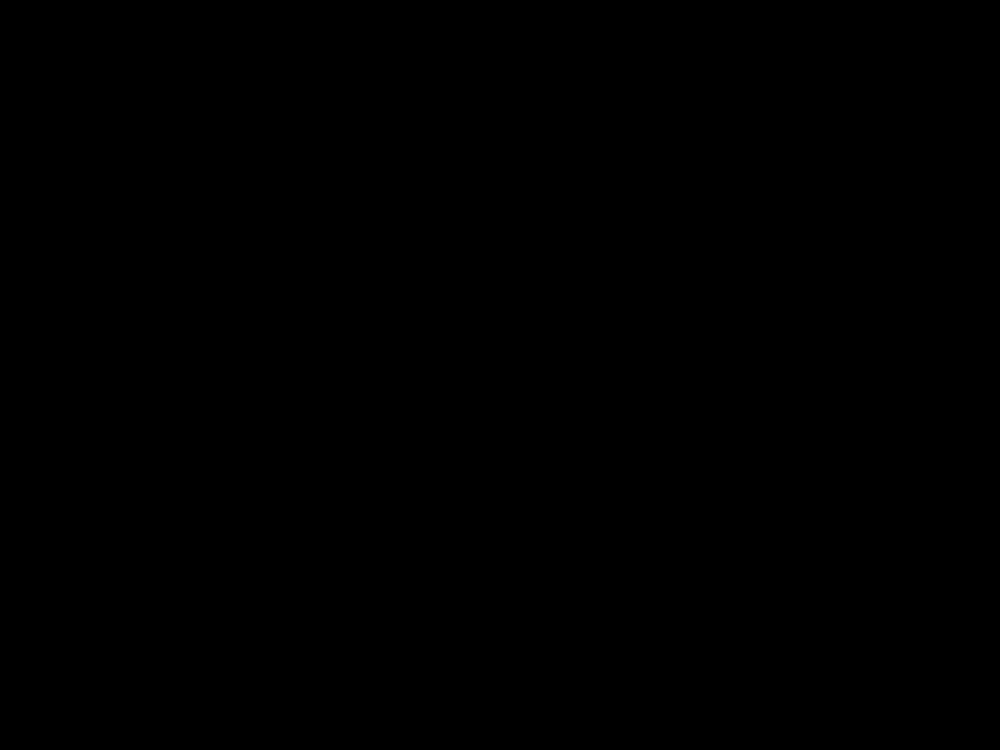
\includegraphics[width=30mm]{images/placeholder.png}}}%
%   \qquad
%   \subfloat[caption 2]{{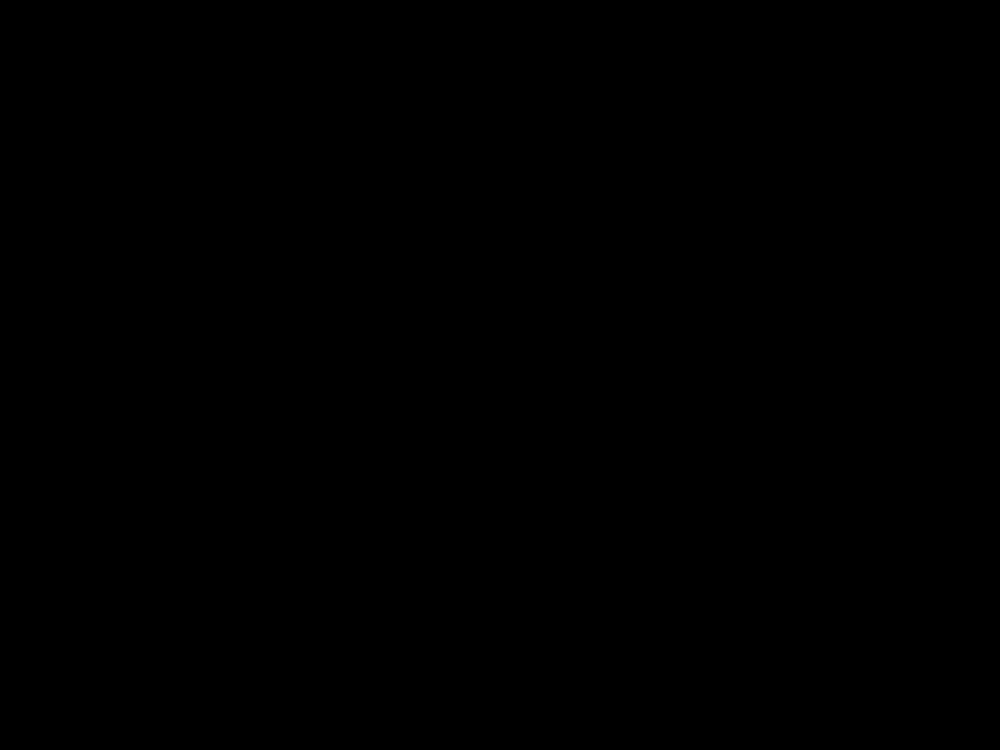
\includegraphics[width=30mm]{images/placeholder.png}}}%
%   \caption{Description}
% \end{figure}

% \begin{figure}[h]
%   \centerline{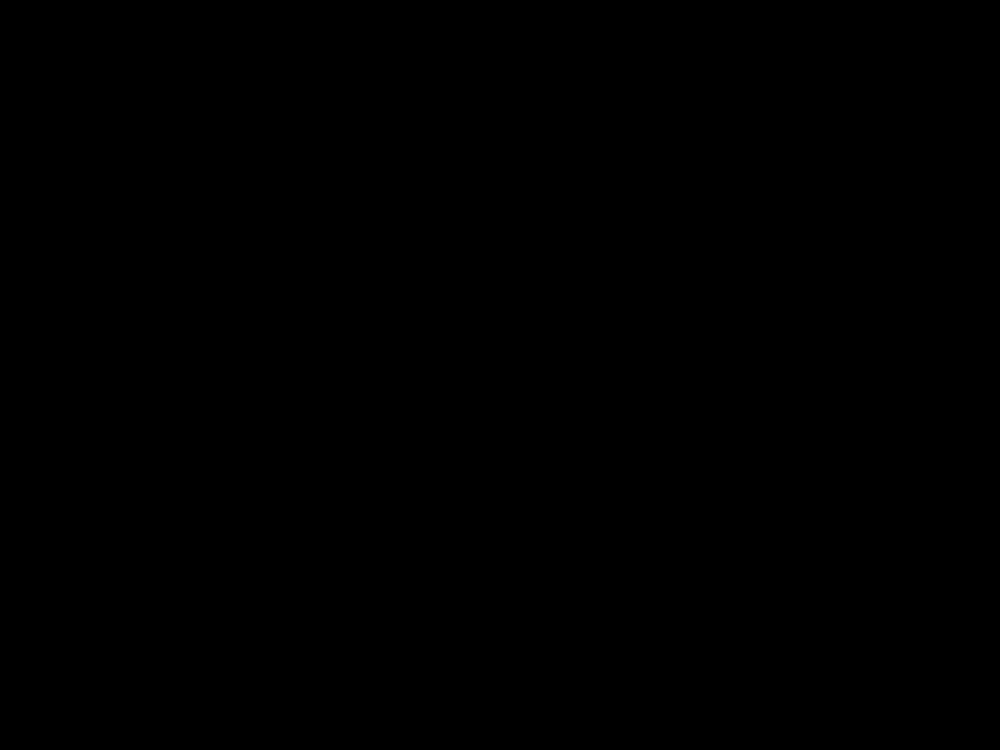
\includegraphics[width=50mm]{images/placeholder.png}}
%   \caption{Description}
% \end{figure}

%Template for a simple table 
%\begin{table}[h]
%   \caption{Description} %title of the table
%   \centering % centering table
%   \begin{tabular}{l rr} % creating three columns
%     \hline\hline %inserting double-line
%     & & \\ [0.5ex] % Insert half line vertical spacing
%     \hline % inserts single-line
%     & & \\ 
%     & & \\
%     & & \\
%     & & \\
%   \hline % inserts single-line
%   \end{tabular}
%   \label{tab:hresult}
% \end{table}
%-----------------------------------------------

\begin{document}
\setcounter{section}{9}
\setcounter{equation}{0}
\section{Thermofluids Lecture 10: The second law of thermodynamics (Part 2) (20/05/2020)}


\subsection{Recap: Entropy}
Entropy is a state variable. The change in entropy of an internally reversible process is given by:
\begin{equation}
  \Delta S = S_2 - S_1 = \left( \int_1^2 \frac{\delta Q}{T} \right)_{b, int\;rev} 
\end{equation}
Unlike mass and energy entropy is not a conserved property. Instead entropy (in the presence of irreversibilities) is generated during a process. For a closed system:
\begin{equation}
  \Delta S = S_2 - S_1 = \left( \int_1^2 \frac{\delta Q}{dT} \right)_b + \sigma
\end{equation}
Where $\sigma$ is the entropy generated during the process (sometimes denoted as $S_{gen}$ instead). The following properties apply to $\sigma$:
\begin{equation}
  \sigma
  \begin{cases}
    = 0,\;\text{no irreversibilities}\\
    > 0,\;\text{irreversibilities present}\\
    < 0,\;\text{impossible process}
  \end{cases}
\end{equation}
The entropy for a cycle is given by a cyclical integral:
\begin{equation}
  \oint \left(\frac{\delta Q}{dT} \right)_b = -\sigma_{cycle}
\end{equation}
It can also be expressed as the discrete sum of $i$ individual steps in the process. The expression then changes to:
\begin{equation}
  \sum_i \frac{\Delta Q_i}{T} = -\sigma_{cycle}
\end{equation}


\subsection{The third law of thermodynamics}
\begin{equation}
  S(T=0\,K, p) = S(T=0\,K) = 0\,J/K
\end{equation}
\textit{Entropy of a system approaches $0$ as temperature of a system approaches absolute $0$.}
Sidenote: The third law is not a definiton, but instead a finding based on how we found entropy to work.


\subsection{Combining the first and second law}
Assuming and ideal system we know that work and heat transfer of energy can be expressed with the following equations:
\begin{gather}
  \delta W = p\,dV\\
  \delta Q = T\,dS
\end{gather}
Thus:
\begin{equation}
  dU = \delta Q - \delta W = T\,dS - p\,dV
\end{equation}
We can rewrite this expression as:
\begin{equation}
  T\,dS = dU + p\,dV \Rightarrow dS = \frac{1}{T}\,dU + \frac{p}{T}\,dV
\end{equation}
We established earlier that $dU = mc_v\,dT$ and we know from the ideal gas eqaution of state that $pV = m\bar{R}T$. Thus when we integrate between states 1 and 2 we end up with:
\begin{equation}
  S_2 - S_1 = \int_1^2 \frac{mc_v}{T}\,dT + \int_1^2 \frac{m\bar{R}}{V}\,dV
\end{equation}
Thus the change in entropy is given as:
\begin{equation}
  S_2(T_2, V_2) - S_1(T_1, V_1) = \int_1^2 \frac{c_v(T)}{T}\,dT + m\bar{R}\ln\left(\frac{V_2}{V_1}\right)
\end{equation}
Now consider enthalpy: $H = U + pV$. Taking the differential of this gives:
\begin{equation}
  dH = dU + d(pV) = dU + p\,dV + V\,dp
\end{equation}
Or written in terms of difference in internal energy:
\begin{equation}
  dU = dH - p\,dV - V\,dp
\end{equation}
We can subsitute this back into our expression of the first law in differential form:
\begin{gather}
  dH - p\,dV - V\,dp = T\,dS - p\,dV \notag\\
  dH = T\,dS + V\,dP
\end{gather}
We know that $dH = mc_p\,dT$. Using the ideal gas equation of state again and integrating we end up with:
\begin{equation}
  S_2 - S_1 = \int_1^2 \frac{mc_p}{T}\,dT + \int_1^2 \frac{m\bar{R}}{p}\,dp
\end{equation}
The change in entropy is then given by:
\begin{equation}
  S_2(T_2, p_2) - S_1(T_1, p_1) = \int_1^2 \frac{c_p(T)}{T}\,dT + m\bar{R}\ln\left(\frac{p_2}{p_1}\right)
\end{equation}
From this we can derrive that systems must be adiabatic if $dS = 0$ since this directly implies there is no energy transfer by heat away from or into the system. In some cases the heat capacity can be approximated as constant. This greatly simplifies the math at the cost of some loss in accuracy. When assuming $c_p$ and $c_v$ to be constant we can rewrite our equations as follows:
\begin{gather}
  s_2(T_2, p_2) - s_1(T_1, p_1) = c_p\ln\left( \frac{T_2}{T_1} \right) - \bar{R}\ln\left( \frac{p_2}{p_1} \right)\\
  s_2(T_2, v_2) - s_1(T_1, v_1) = c_v\ln\left( \frac{T_2}{T_1} \right) - \bar{R}\ln\left( \frac{v_2}{v_1} \right)
\end{gather}
In reality heat capacity is often a function of temperature (there are exceptions such as helium). Having to carry out the intgeral for the heat capacity every time would quickly become cumbersome and is very prone to errors. To circumvent this we define a new variable: $s^\circ$. We calculate the integrals for some specific temperature $T$ and tabulate the results:
\begin{equation}
  s^\circ = \int_0^T \frac{c_p(T)}{T}\,dT \Rightarrow s_2^\circ - s_1^\circ = \int_1^2 \frac{c_p(T)}{T}\,dT
\end{equation}
The values for $s^\circ$ can be found in tables or databases such as coolprop. Subsituting this back into our original equations leaves us with:
\begin{gather}
  s_2(T_2, p_2) - s_1(T_1, p_1) = s_2^\circ - s_1^\circ - \bar{R}\ln\left(\frac{p_2}{p_1} \right)\\
  s_2(T_2, v_2) - s_1(T_1, v_1) = s_2^\circ - s_1^\circ - \bar{R}\ln\left(\frac{v_2}{v_1} \right)\\
\end{gather}


\subsection{$T-S$ diagrams}
Much like a $p-V$ diagram we can draw a $T-S$ diagram to easily visualize a process. Recall the $p-V$ diagram for a Carnot-cycle. The $T-S$ diagram is show below for the same carnot cycle. We know that for an adiabatic internally reversible process $S=$Const.
\begin{figure}[h]
  \centering
  \subfloat[$p-V$ diagram]{{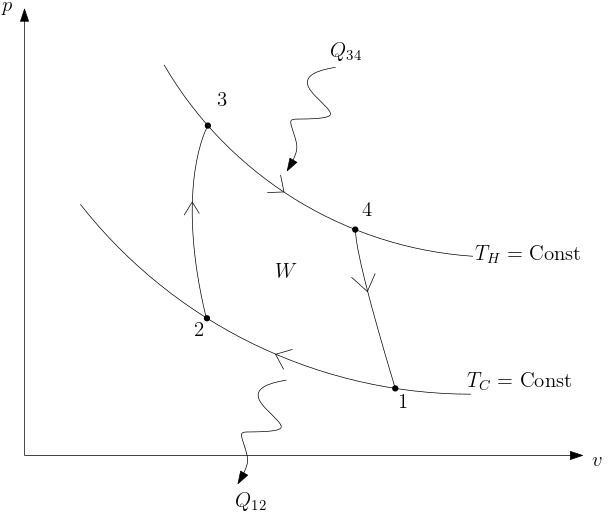
\includegraphics[width=60mm]{images/Carnot Cycle.png}}}%
  \qquad
  \subfloat[$T-S$ diagram]{{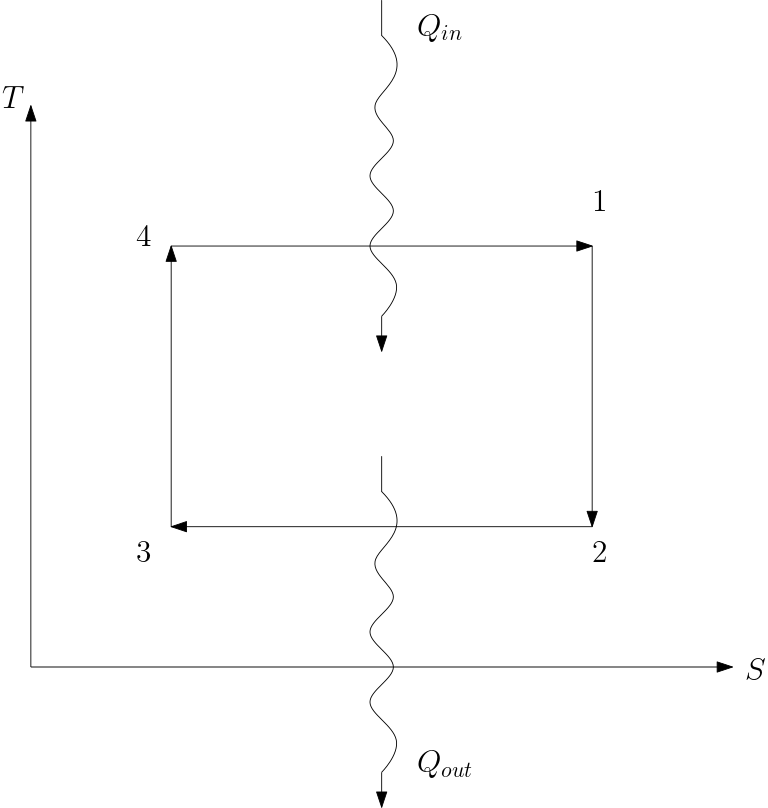
\includegraphics[width=60mm]{images/Carnot Cycle 2.png}}}%
  \caption{The $p-V$ diagram and the $T-S$ diagram of a Carnot cycle.}
\end{figure}
Since the process is internally reversible we know the follwing:
\begin{equation}
  Q_{cycle} = W_{cycle}
\end{equation}
Note that for such a cycle the integral $\int_1^2 T\,dS$ is much easier to compute then the discrete sum of several integrals in the $p-V$ diagram. Thus computing the total work done by the system using a $T-S$ diagram is much, much easier and faster.


\subsection{Entropy balance for open systems}
For open systems we need to take into account that mass can trasnfer entropy into and out of the system. The entropy balance of some control volume is given as:
\begin{equation}
  \frac{dS_{CV}}{dt} = \sum_j \frac{\dot{Q}_j}{T} + \sum_{in} \dot{m}_{in}s_{in} - \sum_{out} \dot{m}_{out}s_{out} + \dot{\sigma}_{CV}
\end{equation}
For stationary processes with 1 inlet and outlet:
\begin{equation}
  \int\left(\frac{\delta Q}{T}\right)_b + \dot{m}(s_{in} - s_{out}) + \dot{\sigma} = 0
\end{equation}


\subsection{Example problem}
\textit{In a closed system $1\,kg$ of air is reversibly compressed from $1\,bar$ and $300\,K$ to $5\,bar$ and $400\,K$. Is this process adiabatic?}
We know the process is reversible, thus $\sigma = 0$. We want to know whether the system is adiabatic or not. If it where $\delta Q = 0$. Since $\delta Q = T\,dS$ this would imply that $dS = 0$. Thus the system is adiabatic if the change in entropy is exactly $0$.
We first solve by assuming $c_p(T) \neq$Const.
\begin{equation*}
  s(T_2, p_2) - s(T_1, p_1) = \int_1^2 \frac{c_p(T)}{T}\,dT - \bar{R}\ln\left( \frac{p_2}{p_1} \right)
\end{equation*}
We know from earlier that $\int_1^2 \frac{c_p(T)}{T}\,dT = s_2^\circ - s_1^\circ$. We also know that $\bar{R} = \frac{R}{M} = \frac{8.3145\,J/molK}{0.02897\,kg/mol} = 287\,J/kgK$. Using a table we find that $s^\circ(T_2) = 1.99194\,kJ/kgK$ and $s^\circ(T_1) = 1.70203\,kJ/kgK$. The expression for $s_2 - s_1$ then becomes:
\begin{align*}
  s_2 - s_1 &= 1.99194\,kJ/kgK - 1.70203\,kJ/kgK - 0.287\,kJ/kgK\cdot \ln\left( \frac{5(10^5)\,Pa}{1(10^5)\,Pa} \right)\\
  &= -0.1720\,kJ/kg
\end{align*}
So the process is in fact not adiabatic, since $dS \neq 0$. The negative value implies heat is leaving the system.\\
We can repeat the problem by instead assuming $c_p(T)=$Const. This would give the following expression:
\begin{equation*}
  s_2 - s_1 = c_p\ln\left(\frac{T_2}{T_1}\right) - \bar{R}\ln\left(\frac{p_2}{p_1}\right)
\end{equation*}
Using the following code in Python and the Coolprop database:
\begin{figure}[h]
  \centerline{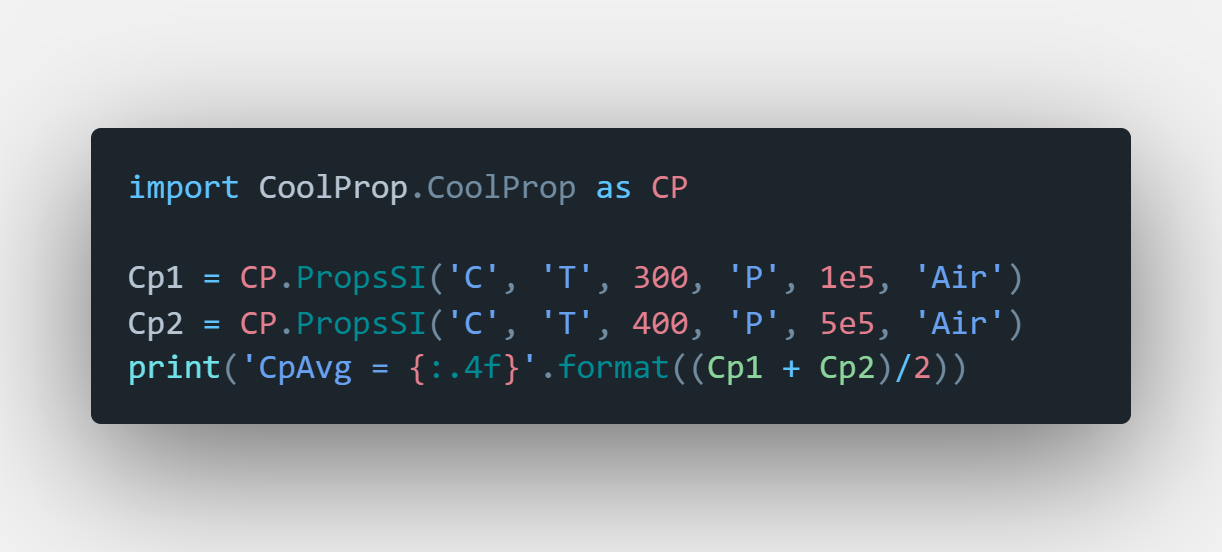
\includegraphics[width=80mm]{images/code.png}}
  \caption{The code used in coolprop to find the value for average heat capacity between $T_1$ and $T_2$.}
\end{figure}
We find that $c_{p, avg} \approx 1.012\,kJ/kgK$. Using this value and filling in the equation we get:
\begin{align*}
  s_2 - s_1 &= 1.012\,kJ/kgK\ln\left(\frac{400\,K}{300\,K}\right) - 0.287\,kJ/kgK\ln\left( \frac{5(10^5)\,Pa}{1(10^5)\,Pa}\right)
  &= -0.1707\,kJ/kgK
\end{align*}
Which is approximatly the same answer. This shows that assuming $c_p$ to be constant is not a bad approximation to make in certain cases.
\end{document}